% Created by tikzDevice version 0.8.1 on 2015-09-15 13:20:22
% !TEX encoding = UTF-8 Unicode
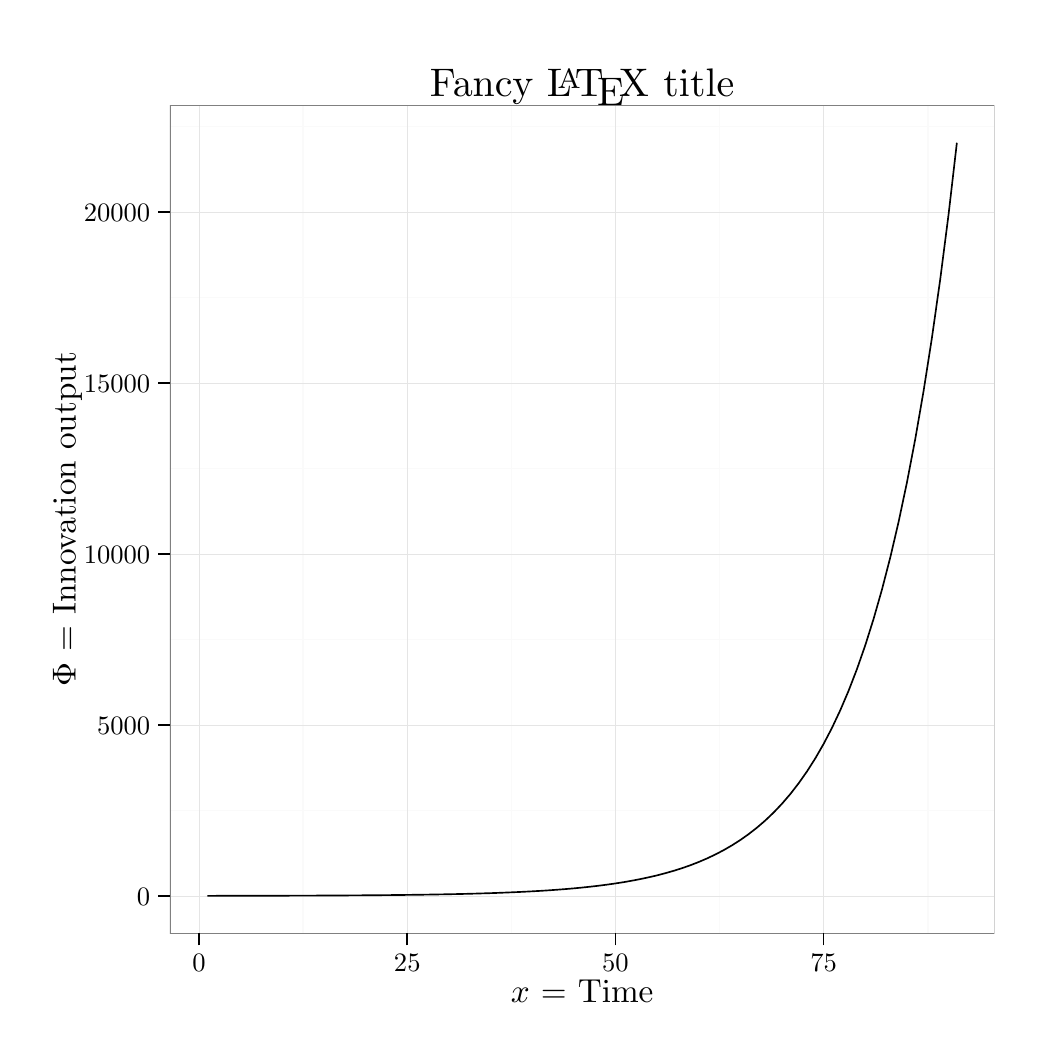
\begin{tikzpicture}[x=1pt,y=1pt]
\definecolor{fillColor}{RGB}{255,255,255}
\path[use as bounding box,fill=fillColor,fill opacity=0.00] (0,0) rectangle (361.35,361.35);
\begin{scope}
\path[clip] (  0.00,  0.00) rectangle (361.35,361.35);
\definecolor{drawColor}{RGB}{255,255,255}
\definecolor{fillColor}{RGB}{255,255,255}

\path[draw=drawColor,line width= 0.6pt,line join=round,line cap=round,fill=fillColor] (  0.00,  0.00) rectangle (361.35,361.35);
\end{scope}
\begin{scope}
\path[clip] ( 51.42, 34.03) rectangle (349.30,333.36);
\definecolor{fillColor}{RGB}{255,255,255}

\path[fill=fillColor] ( 51.42, 34.03) rectangle (349.31,333.36);
\definecolor{drawColor}{gray}{0.98}

\path[draw=drawColor,line width= 0.6pt,line join=round] ( 51.42, 78.50) --
	(349.30, 78.50);

\path[draw=drawColor,line width= 0.6pt,line join=round] ( 51.42,140.27) --
	(349.30,140.27);

\path[draw=drawColor,line width= 0.6pt,line join=round] ( 51.42,202.05) --
	(349.30,202.05);

\path[draw=drawColor,line width= 0.6pt,line join=round] ( 51.42,263.83) --
	(349.30,263.83);

\path[draw=drawColor,line width= 0.6pt,line join=round] ( 51.42,325.61) --
	(349.30,325.61);

\path[draw=drawColor,line width= 0.6pt,line join=round] ( 99.56, 34.03) --
	( 99.56,333.36);

\path[draw=drawColor,line width= 0.6pt,line join=round] (174.78, 34.03) --
	(174.78,333.36);

\path[draw=drawColor,line width= 0.6pt,line join=round] (250.01, 34.03) --
	(250.01,333.36);

\path[draw=drawColor,line width= 0.6pt,line join=round] (325.23, 34.03) --
	(325.23,333.36);
\definecolor{drawColor}{gray}{0.90}

\path[draw=drawColor,line width= 0.2pt,line join=round] ( 51.42, 47.61) --
	(349.30, 47.61);

\path[draw=drawColor,line width= 0.2pt,line join=round] ( 51.42,109.39) --
	(349.30,109.39);

\path[draw=drawColor,line width= 0.2pt,line join=round] ( 51.42,171.16) --
	(349.30,171.16);

\path[draw=drawColor,line width= 0.2pt,line join=round] ( 51.42,232.94) --
	(349.30,232.94);

\path[draw=drawColor,line width= 0.2pt,line join=round] ( 51.42,294.72) --
	(349.30,294.72);

\path[draw=drawColor,line width= 0.2pt,line join=round] ( 61.95, 34.03) --
	( 61.95,333.36);

\path[draw=drawColor,line width= 0.2pt,line join=round] (137.17, 34.03) --
	(137.17,333.36);

\path[draw=drawColor,line width= 0.2pt,line join=round] (212.40, 34.03) --
	(212.40,333.36);

\path[draw=drawColor,line width= 0.2pt,line join=round] (287.62, 34.03) --
	(287.62,333.36);
\definecolor{drawColor}{RGB}{0,0,0}

\path[draw=drawColor,line width= 0.6pt,line join=round] ( 64.96, 47.64) --
	( 67.97, 47.64) --
	( 70.98, 47.65) --
	( 73.98, 47.65) --
	( 76.99, 47.66) --
	( 80.00, 47.66) --
	( 83.01, 47.67) --
	( 86.02, 47.67) --
	( 89.03, 47.68) --
	( 92.04, 47.69) --
	( 95.05, 47.70) --
	( 98.06, 47.71) --
	(101.07, 47.72) --
	(104.07, 47.73) --
	(107.08, 47.74) --
	(110.09, 47.76) --
	(113.10, 47.77) --
	(116.11, 47.79) --
	(119.12, 47.81) --
	(122.13, 47.83) --
	(125.14, 47.86) --
	(128.15, 47.88) --
	(131.15, 47.91) --
	(134.16, 47.94) --
	(137.17, 47.98) --
	(140.18, 48.02) --
	(143.19, 48.06) --
	(146.20, 48.11) --
	(149.21, 48.16) --
	(152.22, 48.22) --
	(155.23, 48.28) --
	(158.24, 48.35) --
	(161.24, 48.43) --
	(164.25, 48.52) --
	(167.26, 48.61) --
	(170.27, 48.72) --
	(173.28, 48.84) --
	(176.29, 48.97) --
	(179.30, 49.11) --
	(182.31, 49.27) --
	(185.32, 49.44) --
	(188.33, 49.63) --
	(191.33, 49.85) --
	(194.34, 50.08) --
	(197.35, 50.34) --
	(200.36, 50.63) --
	(203.37, 50.95) --
	(206.38, 51.30) --
	(209.39, 51.69) --
	(212.40, 52.12) --
	(215.41, 52.59) --
	(218.41, 53.12) --
	(221.42, 53.70) --
	(224.43, 54.34) --
	(227.44, 55.04) --
	(230.45, 55.83) --
	(233.46, 56.69) --
	(236.47, 57.64) --
	(239.48, 58.70) --
	(242.49, 59.87) --
	(245.50, 61.16) --
	(248.50, 62.58) --
	(251.51, 64.16) --
	(254.52, 65.90) --
	(257.53, 67.82) --
	(260.54, 69.95) --
	(263.55, 72.30) --
	(266.56, 74.89) --
	(269.57, 77.76) --
	(272.58, 80.93) --
	(275.59, 84.44) --
	(278.59, 88.31) --
	(281.60, 92.59) --
	(284.61, 97.32) --
	(287.62,102.55) --
	(290.63,108.33) --
	(293.64,114.72) --
	(296.65,121.78) --
	(299.66,129.58) --
	(302.67,138.20) --
	(305.67,147.73) --
	(308.68,158.26) --
	(311.69,169.89) --
	(314.70,182.75) --
	(317.71,196.97) --
	(320.72,212.68) --
	(323.73,230.04) --
	(326.74,249.22) --
	(329.75,270.43) --
	(332.76,293.86) --
	(335.76,319.76);
\definecolor{drawColor}{gray}{0.50}

\path[draw=drawColor,line width= 0.6pt,line join=round,line cap=round] ( 51.42, 34.03) rectangle (349.31,333.36);
\end{scope}
\begin{scope}
\path[clip] (  0.00,  0.00) rectangle (361.35,361.35);
\definecolor{drawColor}{RGB}{0,0,0}

\node[text=drawColor,anchor=base east,inner sep=0pt, outer sep=0pt, scale=  0.96] at ( 44.30, 44.30) {0};

\node[text=drawColor,anchor=base east,inner sep=0pt, outer sep=0pt, scale=  0.96] at ( 44.30,106.08) {5000};

\node[text=drawColor,anchor=base east,inner sep=0pt, outer sep=0pt, scale=  0.96] at ( 44.30,167.86) {10000};

\node[text=drawColor,anchor=base east,inner sep=0pt, outer sep=0pt, scale=  0.96] at ( 44.30,229.64) {15000};

\node[text=drawColor,anchor=base east,inner sep=0pt, outer sep=0pt, scale=  0.96] at ( 44.30,291.41) {20000};
\end{scope}
\begin{scope}
\path[clip] (  0.00,  0.00) rectangle (361.35,361.35);
\definecolor{drawColor}{RGB}{0,0,0}

\path[draw=drawColor,line width= 0.6pt,line join=round] ( 47.15, 47.61) --
	( 51.42, 47.61);

\path[draw=drawColor,line width= 0.6pt,line join=round] ( 47.15,109.39) --
	( 51.42,109.39);

\path[draw=drawColor,line width= 0.6pt,line join=round] ( 47.15,171.16) --
	( 51.42,171.16);

\path[draw=drawColor,line width= 0.6pt,line join=round] ( 47.15,232.94) --
	( 51.42,232.94);

\path[draw=drawColor,line width= 0.6pt,line join=round] ( 47.15,294.72) --
	( 51.42,294.72);
\end{scope}
\begin{scope}
\path[clip] (  0.00,  0.00) rectangle (361.35,361.35);
\definecolor{drawColor}{RGB}{0,0,0}

\path[draw=drawColor,line width= 0.6pt,line join=round] ( 61.95, 29.77) --
	( 61.95, 34.03);

\path[draw=drawColor,line width= 0.6pt,line join=round] (137.17, 29.77) --
	(137.17, 34.03);

\path[draw=drawColor,line width= 0.6pt,line join=round] (212.40, 29.77) --
	(212.40, 34.03);

\path[draw=drawColor,line width= 0.6pt,line join=round] (287.62, 29.77) --
	(287.62, 34.03);
\end{scope}
\begin{scope}
\path[clip] (  0.00,  0.00) rectangle (361.35,361.35);
\definecolor{drawColor}{RGB}{0,0,0}

\node[text=drawColor,anchor=base,inner sep=0pt, outer sep=0pt, scale=  0.96] at ( 61.95, 20.31) {0};

\node[text=drawColor,anchor=base,inner sep=0pt, outer sep=0pt, scale=  0.96] at (137.17, 20.31) {25};

\node[text=drawColor,anchor=base,inner sep=0pt, outer sep=0pt, scale=  0.96] at (212.40, 20.31) {50};

\node[text=drawColor,anchor=base,inner sep=0pt, outer sep=0pt, scale=  0.96] at (287.62, 20.31) {75};
\end{scope}
\begin{scope}
\path[clip] (  0.00,  0.00) rectangle (361.35,361.35);
\definecolor{drawColor}{RGB}{0,0,0}

\node[text=drawColor,anchor=base,inner sep=0pt, outer sep=0pt, scale=  1.20] at (200.36,  9.03) {$x$ = Time};
\end{scope}
\begin{scope}
\path[clip] (  0.00,  0.00) rectangle (361.35,361.35);
\definecolor{drawColor}{RGB}{0,0,0}

\node[text=drawColor,rotate= 90.00,anchor=base,inner sep=0pt, outer sep=0pt, scale=  1.20] at ( 17.30,183.70) {$\Phi$ = Innovation output};
\end{scope}
\begin{scope}
\path[clip] (  0.00,  0.00) rectangle (361.35,361.35);
\definecolor{drawColor}{RGB}{0,0,0}

\node[text=drawColor,anchor=base,inner sep=0pt, outer sep=0pt, scale=  1.44] at (200.36,336.38) {Fancy \LaTeX  \hspace{0.01cm} title};
\end{scope}
\end{tikzpicture}
